\section{Zielsetzung}
In diesem Versuch soll das Geiger-Müller-Zählrohr untersucht werden.
Ein Geiger-Müller-Zählrohr ist ein Instrument zur Messung von ionisierender Strahlung.
Im folgenden werden die Kenndaten eines Zählrohrs, wie Totzeit oder Plateau-Anstieg ermittelt.



\section{Theoretische Grundlagen}
\subsection{Aufbau und Wirkungsweise}

\noindent
Ein Geiger-Müller-Zählrohr besteht aus einem Stahlmantel, in dessen Mitte sich ein Anodendraht befindet. Diese beiden sind an eine Spannungsquelle angeschloßen.
Der Zwischenraum ist mit einem Gasgemisch, wie zum Beispiel Argon und Ethylalkohol. Dies ist in Abb.\ref{img:aufbau} noch einmal dargestellt. Der Anodendrahtist dabei an eigenen
Verstärker angeschlossen, wodurch der Impuls von einfallenden Elektronen verstärkt wird.

\begin{figure}[H]
    \centering
    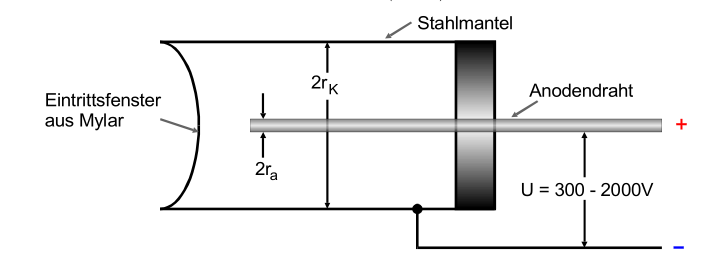
\includegraphics[width=0.75\textwidth]{images/Aufbau.PNG}
    \caption{Der schematische Aufbau eines Geiger-Müller-Zählrohrs \protect \cite{V703}.}
    \label{img:aufbau}
\end{figure}

\noindent
Es gibt verschiedene Prozesse die im inneren des Zählrohrs ablaufen können. 
Welcher Prozess genau stattfindet ist in der Regel abhängig von der Stärke des radialsymmetrischen, elektrischen Feldes im Inneren, und damit von der angelegten Spannung.\\
Die Abhängigkeiten von der Spannung und Art der ionisierenden Strahlung sind in Abb.\ref{img:spannung} aufgetragen.\\\\
In der Regel tritt zuerst ein Teilchen in das Volumen des Zählrohres ein. Dort ionisiert es eine Mengen an Gasteilchen, proportional zu seiner eigenen Energie.\\
Die nachfolgenden Prozesse zeigen jetzt die Spannngsabhängigkeit.\\\\
Bei kleinen angelegten Spannungen, dies ist Bereich \textbf{I} in der Abbildung, erreicht nur ein kleiner Teil, der durch Ionisation erzeugten Elektronen den Anodendraht. 
Dies liegt daran, dass die Beschleunigung der Elektronen im elektrischen Feld so klein ist dass die meisten vorm Eintreffen am Draht rekombinieren. \\\\
Im Bereich \textbf{II}, also bei höheren Feldstärken, verschwindet dieser Effekt. Dort herrscht dann also wirklich eine Proportionalität zwischen der Energie der Strahlung und dem Ionisationsstrom.
Ionisationskammern arbeiten in diesem Bereich. Wegen trotzdem geringer Ionisationsströme ist dieser Bereich nur bei hoher Strahlungsintensität wirksam.\\\\
Bei noch höheren Spannungen, wie im Bereich \textbf{III}, werden die Elektronen im Feld sogar so stark beschleunigt, dass sie selber weitere Stoßionisationen hervorrufen.
Dieser Effekt kann sich lawinenartig fortführen, weswegen das ganze auch Townsend-Lawine genannt wird. 
Ein hier operierendes Messinstrument wird Proportonalitätszählrohr genannt.\\\\
Der Bereich \textbf{IV} ist allerdings erst der eigentliche Operationsbereich des Zählrohres. 
Dort ist keine direkte Proportionalität zwischen der primären Energie der Strahlung und den gemessenen Ladungsimpulsen mehr gegeben.\\
Dies lässt sich darauf zurückführen, dass bei den Ionisationen zusätzlich UV-Photonen entstehen.
Diese breiten sich, vom elektrischen Feld nicht beeinflusst, im Volumen des Zählrohres aus und führen dort zu weiteren Ionisationen.
Die Größe des Ladungsimpulses ist jetzt nur noch vom Volumen des Rohres und der Spannung abhängig.
Diese Effekte sind einfach nachzuweisen, lassen sich aber nur noch für eine Intensitätsmessung nutzen.\\\\
Die nachfolgende Abbildung stellt noch einmal die einzelnen Bereiche grafisch dar.

\begin{figure}[H]
    \centering
    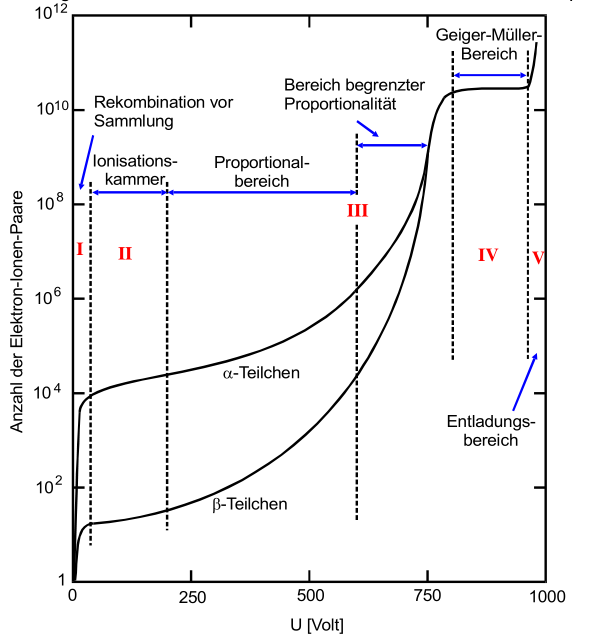
\includegraphics[width=0.75\textwidth]{images/Spannungsgrafik.PNG}
    \caption{Ein Diagramm welches die Abhängigkeit der gemessenen Elektronen-Ionen-Paare im Verhältnis zur Spannung und Strahlngsart abbildet. \protect \cite{V703}.}
    \label{img:spannung}
\end{figure}


\subsection{Totzeit und Nachentladungen}


\noindent
Die Elektronen bewegen sich relativ schnell zur Anode um dort abzuwandern. Die Ionen hingegen, welche eine große Masse besitzen brauchen dafür deutlich länger.
Dies führt dazu, dass die Ionen einen radialsymmetrischen Bereich um sich selbst bilden in dem das E-Feld teilweise aufgehoben wird. Mehrere Ionen bilden dann, entlang der Bahn eines Teilchens, einen so genannten Ionenschlauch.\\
Dieser Ionenschlauch veringert, für eine Zeit $T$, das E-Feld soweit, dass keine Stoßionisationen mehr stattfinden können. Diese Zeit nennt man Totzeit.\\
Während die verantwortlichen Ionen abtranstportiert werden können schon wieder einige wenige Stoßionisationen stattfinden. 
Allerdings nicht in einem Maße wie vor der Entstehung des Schlauches. Diese sich der Totzeit anschließende Zeitintervall nennt sich Erholungszeit $T_E$.\\
Dieser ganze Vorgang wird in der folgenden Abbildung \ref{img:tot} noch einmal grafisch dargestellt.

\begin{figure}[H]
    \centering
    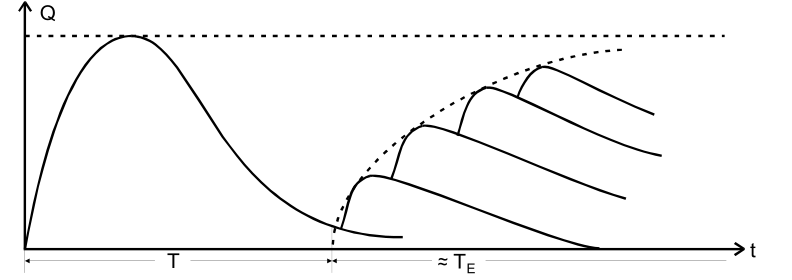
\includegraphics[width=0.6\textwidth]{images/Totozeit.PNG}
    \caption{Die Tot- und Erholungszeit in einem Ladungs-Zeit-Diagramm. Die gestrichelte, einhüllende von $T_E$ lässt sich praktisch nur ungenau bestimmen \protect \cite{V703}.}
    \label{img:tot}
\end{figure}

\noindent
Ionen, welche auf den Mantel des Zählrohres treffen, können bis dahin so beschleunigt worden sein, dass sie die Austrittsarbeit für Elektronen verrichten können.
Diese so genannten Sekundärlektronen werden daraufhin beim durchschreiten der gesamten Spannung wieder so beschleunigt, dass sie, mit der Townsend-Lawine, zu weiteren Impulsen führen.\\
Diesen Vorgang nennt man Nachentladung. Der Zeitraum den sie nach der ursprünglichen Ionisation stattfinden wird mit $T_L$ bezeichnet. Er entspricht ungefähr der Streckendauer der Ionen zum Mantel.\\
Dieser Vorgang ist unerwünscht, da er nach der Totozeit neu eingetretene Teilchen simuliert und so die Messungen verfälscht. \\
Es gibt aber Methoden, wie das hinzugeben von Alkoholdämpfen in das Gasgemisch, die in der Lage sind diesen Effekt zu mindern.
Diese werden dann nämlich auf dem Weg vom Mantel von den Edelgasionen ionisiert. Diese verlieren dadurch ihre kinetische Engergie. 
Des Weiteren sind die Alkohol Ionen nicht Massereich genug um genug Energie zu erhalten um die Austrittsarbeit für die Elektronen zu leisten. Stattdessen führen sie nur zu Schwingungen.\\


\subsection{Charakteristik des Zählrohres}

\noindent
Durch Auftragen einer bestimmten Zahl von Teilchen $N$ bei konstanter Strahlungsintensität 
gegen die Spannung erhält man die folgende Abbildung, welche die Charakteristik des Zählrohres genannt wird.

\begin{figure}[H]
    \centering
    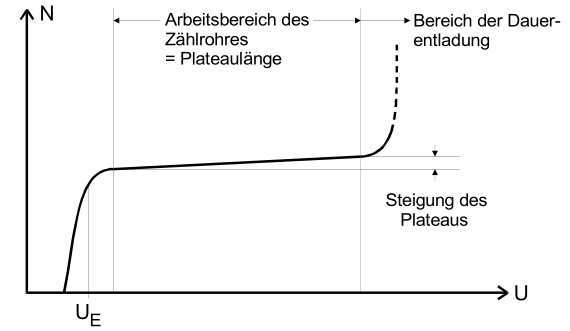
\includegraphics[width=0.6\textwidth]{images/charakteristik.PNG}
    \caption{Die Charakteristik eines Geiger-Müller-Zählrohres \protect \cite{V703}.}
    \label{img:char}
\end{figure}

\noindent
Dabei ist $U_E$ die Spannung bei der die Stoßionisationen beginnen. Der ihr nachfolgende Bereich nennt sich Auslösebereich.\\
Die Steigung des Plateaus ist abhängig von der Effektivität des Alkohols Nachentladungen zu unterdrücken. Würde es keine geben, was praktisch unrealistisch ist, wäre die Plateau Steigung null.
Ein breites und flaches Plateau spricht dabei für die Qualität eines Zählrohres.\\
Der Bereich hinter dem Plateau entsteht durch einzelne Entladungen, die Aufgrund von vorher beschriebenen Vorgängen zu dauerhaften Entladungen führen kann, welche sogar das Zählrohr zerstören können.\\

\subsection{Ansprechvermögen des Zählrohres}

\noindent
Das Ansprechvermögen eines Zählrohres beschreibt die Wahrscheinlichkeit mit der ein einfallendes Teilchen nachgewiesen werden kann.\\
Bei $\alpha$- und $\beta$-Teilchen ist diese Aufgrund ihrer Größe fast $\SI{100}{\percent}$. Das Nadelöhr ist dort eher das eintreten in das Zählrohr. 
Um dieses zu verhindern werden an die Spitze des Rohres zum Beispiel Fenster aus Mylar-Folie angebracht. Diese können von den beiden Teilchenarten gut durchquert werden.
Dies ist auch noch einmal in Abb.\ref{img:aufbau} zu sehen.\\
Das Ansprechvermögen für $\gamma$-Quanten ist in der Größenordung $\SI{1}{\percent}$. Es lässt sich zwar mit schweren Füllgasen wie Xenon erhöhen, liefert allerdings trotzdem nur bei Röntgen-Quanten
oder hohen Intensitäten vernünftige Ergebnisse.

